\chapter{Foundations}

\section{Tools}

\subsection*{Python}

Python is an interpreted, object-oriented, high-level programming language with dynamic semantics.
It is built for Rapid Application Development with and easy to learn syntax for readability.
Key features are built in data structures, dynamic typing and binding.
\cite{python-lang}
It has its own package manager called python Package Index (PyPi).
The language is compiled at execution and is available for all major platforms without charge.
The programming language is open source and maintained by the Pthon Software Foundation.
\cite{python-software-foundation}


\subsection*{NumPy}

NumPy is a package for Python.
It enables scientific computing with N-dimensional array objects and supports array broadcasting, type casting and basic linear algebra functions.
\cite{numpy-package}


\subsection*{Tensorflow}

Tensorflow is an entire ecosystem for solving problems with machine learning.
It is developed and maintained by the Google Brain team.
In 2015 it was released unser the Apache 2.0 open-source license.
It offers multiple levels of abstraction for building, training and testing models.
For more flexibility it allows visualisations of the code and intuitive debugging.
Large machine learning training tasks can be done with distributed training on different hardware configurations without changing the model definition.
Trained models can be directly put into production.
Moreover Tensorflow offers support for multiple languages and platforms.
\cite{tensorflow-about}

\subsubsection*{Core Concepts}

Tensorflow consists of a server client architecture.
The core is located on the server side and developed in C++.
Developers use client liberaries in different languages to interact with the core.
The general architecture for developers of Tensorflow is shown in figure \ref{fig:tensorflow_programming_environment_image}.

\begin{figure}[H]
    \centering
    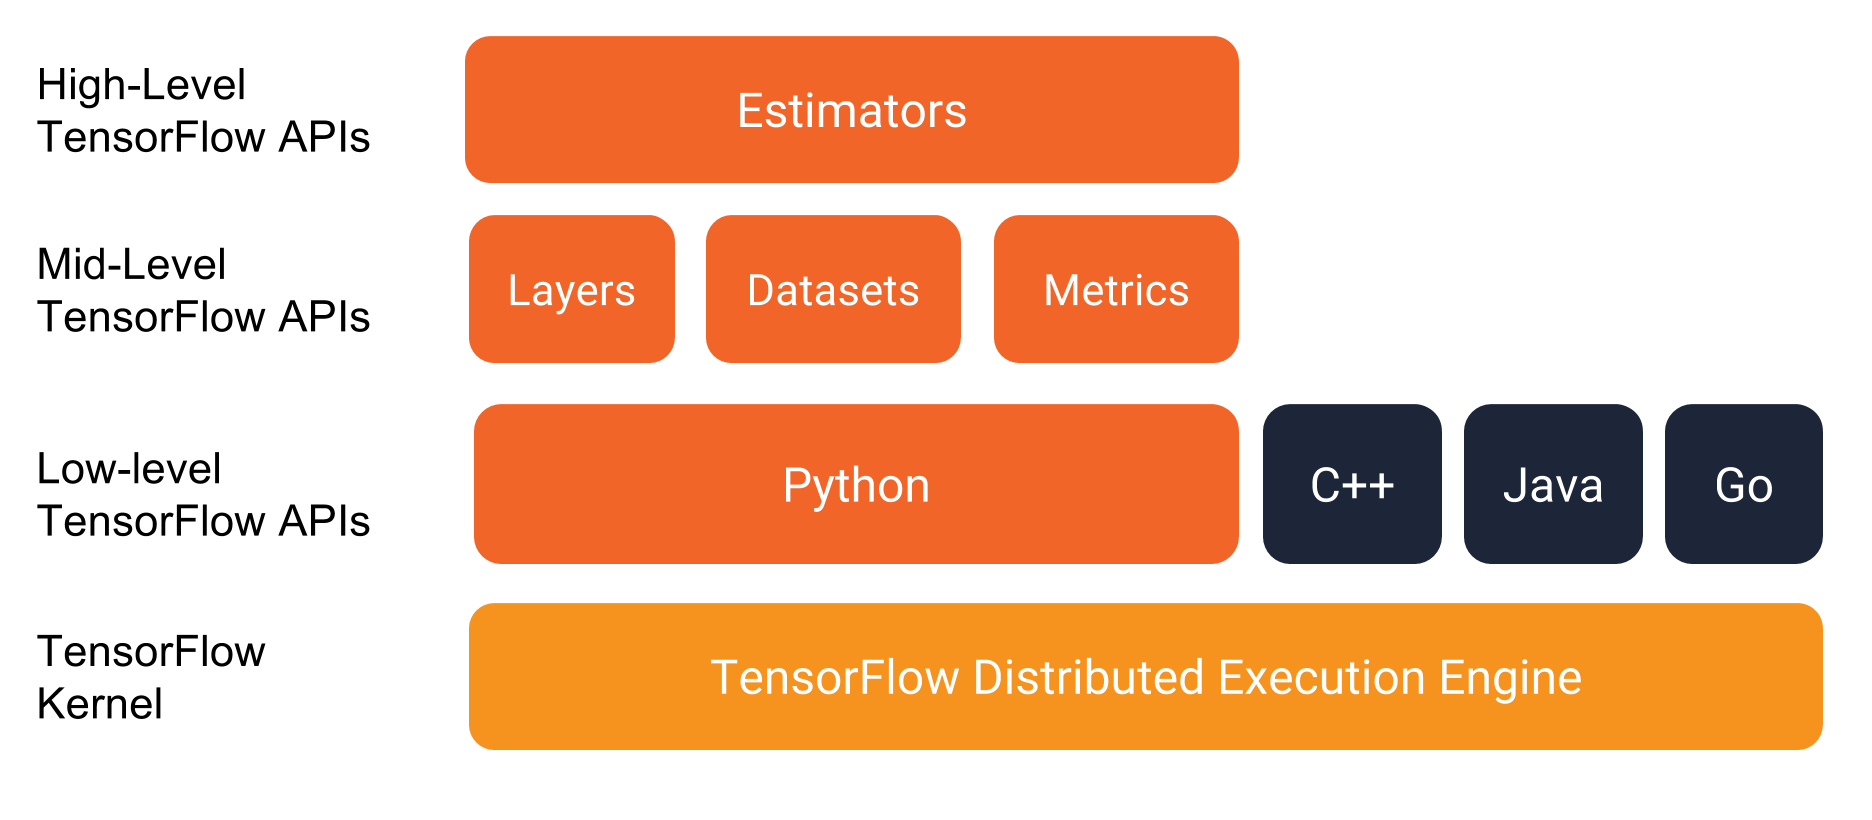
\includegraphics[width=\textwidth]{tensorflow_programming_environment}
    \caption{\cite{tensorflow_programming_environment_image} Tensorflow programming environment}
    \label{fig:tensorflow_programming_environment_image}
\end{figure}

The most important concept for developers is the dataflow graph functionality.
All variables, constants and operations form a computation graph.
Parts of the graph can be started and calculated across a set of local and remote devices.
Figure \ref{fig:tensorflow_graph_image} shows an example of a computation graph:

\begin{figure}[H]
    \centering
    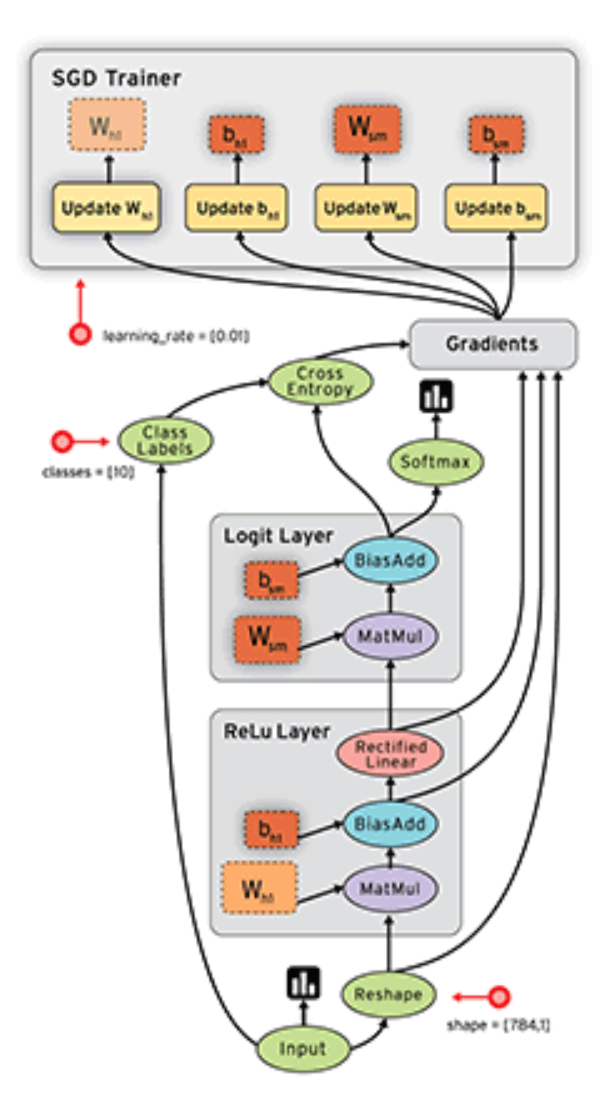
\includegraphics[scale=.5]{tensors_graph}
    \caption{\cite{tensorflow_graph_image} Tensorflow graph}
    \label{fig:tensorflow_graph_image}
\end{figure}

\section{MNIST Dataset}

\begin{figure}[H]
    \centering
    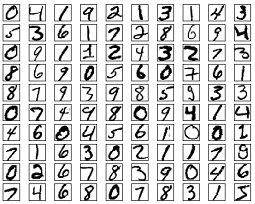
\includegraphics{mnist_100_digits}
    \caption{\cite{mnist_examples_image} Examples of handwritten digits in the mnist dataset}
    \label{fig:mnist_examples}
\end{figure}

The MNIST database is a public available dataset of handwritten digits.
It contains a set of 70,000 entities split into 60,000 training and 10,000 test parts.
The digits are size-normalized and centered photos with a fixed-size of 28 by 28 pixels.
The numbers are created by approximately 250 writers. 
\cite{mnist-database}
The Dataset pertains to one of the most popular dataset for research and testing the performance of new networks.
It is a great resource for testing new deep learning algorithms with supervised learning.

\section{Deep Neural Network}

The Introduction gave a basic overview of the understanding and behind the scenes of a neural network.
This section shows the construct and math of the network used for the elastic weight consolidation implementation and scenario testing.

As described, a neural network is a collection of neurons connected with weights and paired together in layers.
Each neuron receives values from all neurons on the layer before.
Each connection holds a value which represents the importance.
Therefore this connected value is called weight.
The neuron computes all the input values (x) with the weights (w) and applies a bias (b) to predict the result (y).
Figure \ref{fig:dnn_node_procedure} shows the computation structure of each neuron in the network.
\cite{math_nn_skalski}

\begin{figure}[H]
    \centering
    \begin{tikzpicture}[
        init/.style={
        draw,
        circle,
        inner sep=2pt,
        font=\Huge,
        join = by -latex
        },
        squa/.style={
        draw,
        inner sep=2pt,
        font=\Large,
        join = by -latex
        },
        start chain=2,node distance=13mm
        ]
        \node[on chain=2] 
        (x2) {$x_2$};
        \node[on chain=2,join=by o-latex] 
        {$w_2$};
        \node[on chain=2,init] (sigma) 
        {$\displaystyle\Sigma$};
        \node[on chain=2,squa,label=above:{\parbox{2cm}{\centering Activation \\ function}}]
        {$f$};
        \node[on chain=2,label=above:Output,join=by -latex] 
        {$y$};
        \begin{scope}[start chain=1]
            \node[on chain=1] at (0,1.5cm) 
            (x1) {$x_1$};
            \node[on chain=1,label=above:Weights,join=by o-latex] 
            (w1) {$w_1$};
        \end{scope}
        \begin{scope}[start chain=3]
            \node[on chain=3] at (0,-1.5cm) 
            (x3) {$x_3$};
            \node[on chain=3,join=by o-latex] 
            (w3) {$w_3$};
        \end{scope}
        \node[label=above:\parbox{2cm}{\centering Bias \\ $b$}] at (sigma|-w1) (b) {};
        
        \draw[-latex] (w1) -- (sigma);
        \draw[-latex] (w3) -- (sigma);
        \draw[o-latex] (b) -- (sigma);
        
        \draw[decorate,decoration={brace,mirror}] (x1.north west) -- node[left=10pt] {Inputs} (x3.south west);
    \end{tikzpicture}
    \caption{\cite{dnn_neuron_basic_overview} Neuron computation structure}
    \label{fig:dnn_node_procedure}
\end{figure}

The value of each output neuron can be calculated as the following \cite{medium_nn_from_scratch}:

$$y = b + \sum_{i} x_i w_i$$

To be able to ensure the quickest calculation possible, vectorisation and matrixes are used.
All Weights on a layer get stacked to a matrix W together.
The same process is applied to the biases on each layer.
This results in the following calculation
\cite{medium_nn_from_scratch}:

$$ X = [ x_1 \dots x_i ]; \space W = 
\begin{bmatrix}
    x_{11} & \dots  & x_{1j} \\
    \vdots & \ddots & \vdots \\
    x_{i1} & \dots  & x_{ij}
\end{bmatrix}; \space
B = [ b_1 \dots b_j ] $$

\begin{equation}
    Y = X * W + B
\end{equation}

Finally the result of this calculation is passed through an activation function.
This activation function is the key element of a neural network.
Without it, a neural network would just be a combination of linear functions, which can be combined into on linear function.
The activation function modifies the result in a probabilistic way.
Important to mention is, that the activation function has a significant impact on the speed of learning.
The network in this article uses the ReLU as an activation function for the hidden layers \cite{math_nn_skalski,relu}:
$$ReLU(x) = max(0,x)$$

The output of the last layer will be computed as logits:
$$logits = (x*w)+b$$

On the output layer it uses the softmax function, which realtes the output classes in a probabilistic way:
$$ Softmax : \mathbb{R}^K \to \mathbb{R}^K $$
$$ Softmax(x)_i : \frac{e^{k_i}}{\sum_{k=1}^K e^{x_k}}
\space ; i = 1, …, K
$$
$$probabilities = Softmax(logits)$$

After a prediction by the calculation of all neurons and layers the network needs source of information on the progress of the learning process.
This is where the loss function is introduced.
It is designed to show how bad the classification to the right solution is.
In this article the crossentropy loss function is used.
\cite{math_nn_skalski, medium_nn_from_scratch}

$$CrossEntropy(p,y) = -\sum_{i=1}^K y_i \log(p_i)$$
$$loss = CrossEntropy(probs, y)$$

This process of calculating a result of the network is called forward propagation.
It puts an input into the network and it calculates based on the parameters and functions an output.
On this output the learning process gets applied.
This shows the accuracy of the network.
\cite{math_nn_skalski, medium_nn_from_scratch}

The learning process is about adapting the weights and biases to
optimise the accuracy.
This is done by minimising the loss function.
This process of the update of weights and biases is called Backpropagation.
It is an algorithm which calculates error gradients with respect to each network variable.
Those gradients are later used in an optimization algorithm called Gradient Descent.
This method is used to find a function minimum.
After the minimum is found, it would be applied to all parameters in the network.
By adjusting the learning rate of backpropagation, the developer has the control over the value adjustment.
He defines how detailed each learning step should be.
\cite{math_nn_andrey}

Running the Gradient Descent algorithm multiple times on different examples eventually result in a properly trained neural network.

\section{Catastrophic Forgetting}

Catastrophic forgetting was first discovered in 1989 in the article "Catastrophic Intereference" by McCloskey and Cohen.
They broke the problem down into a rather simplified version to explain the problem:
Figure \ref{fig:catastrophic_forgetting_clarification}A shows a reprensentation of a network in a simplified form.
It has stored the facts $5 + 4 = 9$ and $6 + 4 = 10$.
\hfill \break
Now this network wants to learn new facts.
Figure \ref{fig:catastrophic_forgetting_clarification}B shows the appendix of the new fact $7 + 4 = 11$.
To be able to learn this fact it is represented seperate to the representation of other facts.
This storing of facts does not disrupt the representation of presious learned knowledge.
\hfill \break
But in a neural network the representation is quite different.
All weights are involved in responding to many different inputs.
To be able to predict the additional new desired outcome, it has to adjust the weights.
This process will alter the network's response to the other input patterns.
It results in changing weights to encode new information and alters previously learned responses to other inputs.

\begin{figure}[H]
    \centering
    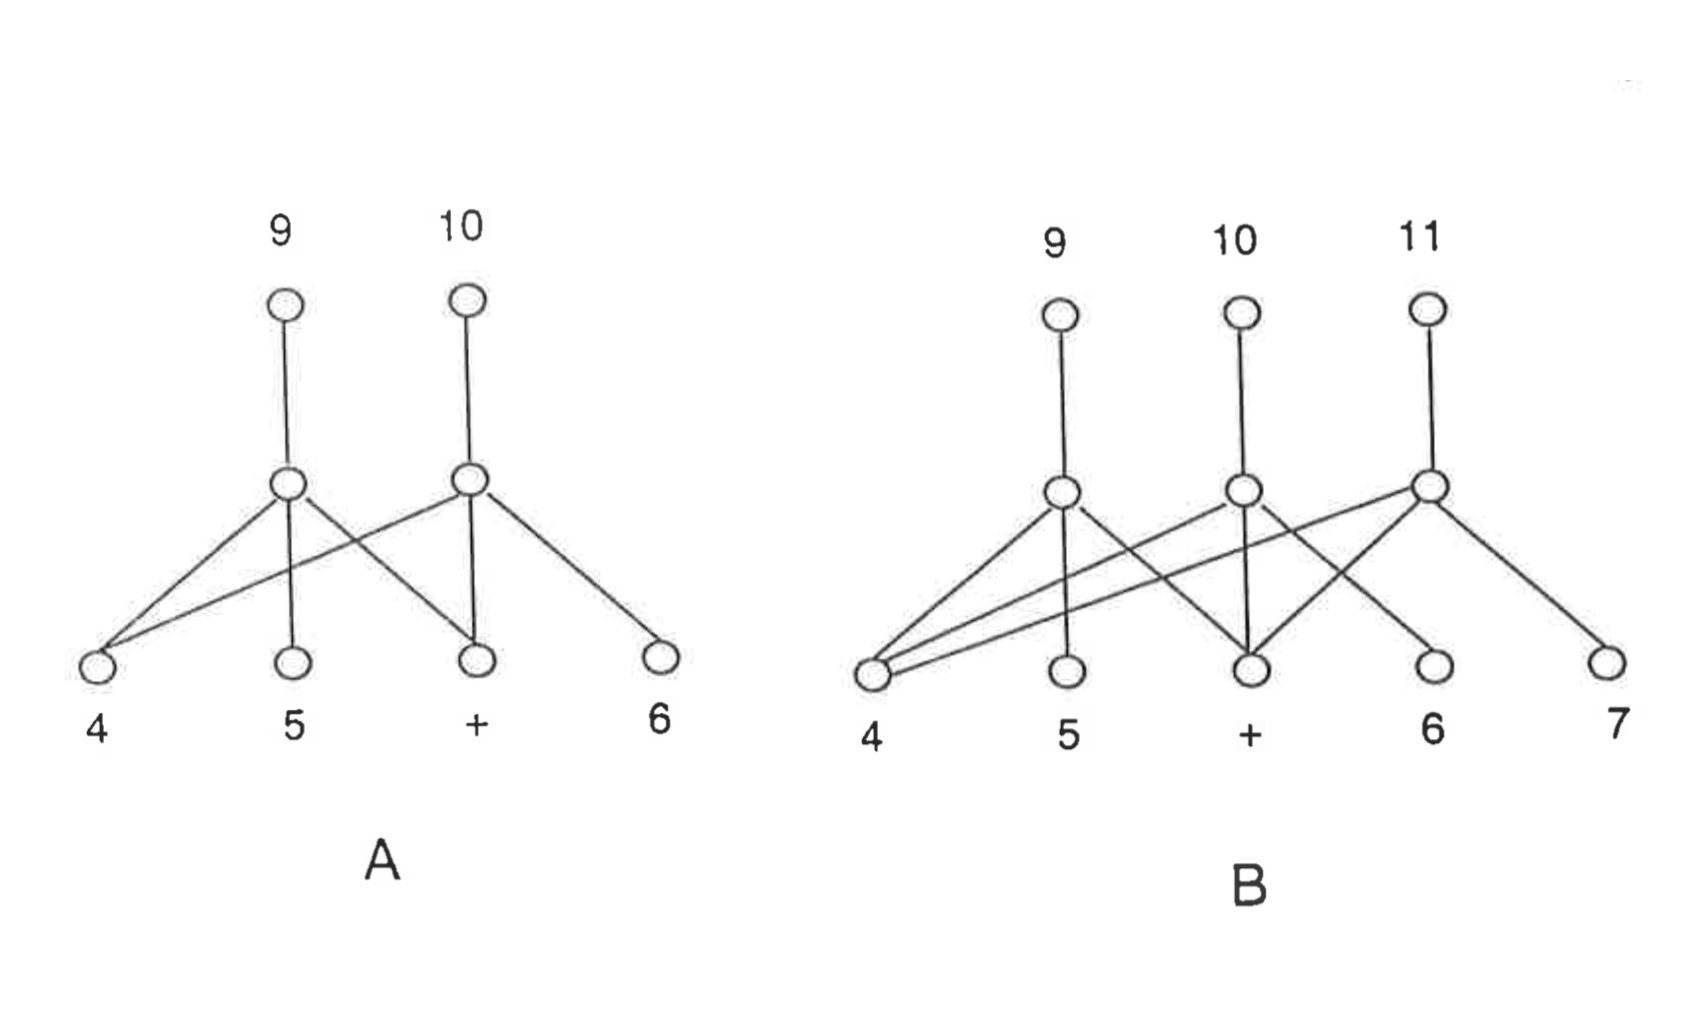
\includegraphics[width=\textwidth]{McCloskeyCohen1989CatastropicInterference}
    \caption{\cite[page 148]{psychology_learning_mccloskey_cohen} Catastrophic forgetting clarification}
    \label{fig:catastrophic_forgetting_clarification}
\end{figure}


\section{Elastic Weight Consolidation}

…